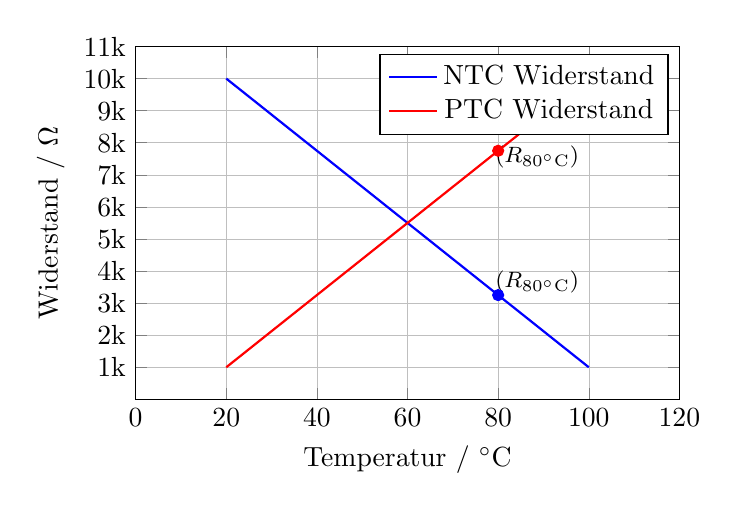
\begin{tikzpicture}
    \begin{axis}[
            xlabel={Temperatur / $^\circ$C},
            ylabel={Widerstand / $\Omega$},
            xmin=0, xmax=120,
            ymin=0, ymax=11000,
            xtick={0,20,...,120},
            ytick={1000,2000,...,11000},
            yticklabels={1k,2k,3k,4k,5k,6k,7k,8k,9k,10k,11k},
            grid=both,
            major grid style={line width=.2pt,draw=gray!50},
            minor grid style={line width=.1pt,draw=gray!20},
            width=0.7\textwidth,
            height=0.5\textwidth,
            scaled y ticks=false
        ]

        % NTC Widerstand
        \addplot[
            color=blue,
            mark=none,
            thick,
        ] coordinates {
                (20,10000)(100,1000)
            };
        \addlegendentry{NTC Widerstand}

        % PTC Widerstand
        \addplot[
            color=red,
            mark=none,
            thick,
        ] coordinates {
                (20,1000)(100,10000)
            };
        \addlegendentry{PTC Widerstand}

        % Punkte auf der Linie markieren
        \addplot[
            color=red,
            only marks,
            mark=*,
            mark size=2pt
        ]coordinates {
        (80,7750)
        };

        % Punkte auf der Linie markieren
        \addplot[
            color=blue,
            only marks,
            mark=*,
            mark size=2pt
        ] coordinates {
                (80,3250)
            };

        % Beschriftungen der Punkte PTC
        \node[anchor=south east, font=\footnotesize] at (axis cs:100,6900) {($R_{\mathrm{80^\circ C}}$)};
        % Beschriftungen der Punkte NTC
        \node[anchor=south east, font=\footnotesize] at (axis cs:100,3000) {($R_{\mathrm{80^\circ C}}$)};

    \end{axis}
\end{tikzpicture}